\documentclass{beamer}

\usepackage{beamerthemesplit}
\usepackage{verbatim}

\usetheme{Pittsburgh}
%\usecolortheme{seagull}
%\usecolortheme{seahorse}
\usecolortheme{beaver}

\usefonttheme{serif}

\newcommand{\snT}{$(S/N)_{\textrm{size}}$}
%\newcommand{\snT}{$\left( \frac{S}{N}\right)_{\textrm{size}}$}
\newcommand{\snflux}{$(S/N)_{\textrm{flux}}$}
%\newcommand{\snflux}{$\left( \frac{S}{N}\right)_{\textrm{flux}}$}

\newcommand{\vecg}{\mbox{\boldmath $g$}}
\newcommand{\vecQ}{\mbox{\boldmath $Q$}}
\newcommand{\matR}{\mbox{$\bf R$}}
\newcommand{\matC}{\mbox{$\bf C$}}
\newcommand{\sersic}{S\'{e}rsic}
\newcommand{\devauc}{De Vaucouleurs'}


\title{Perfecting Weak Lensing Measurements}
\author{Erin Sheldon}
\institute{Brookhaven National Laboratory}

% http://texblog.net/latex-archive/plaintex/beamer-footline-frame-number/
% to add the page (frame ) number and not screw up the bottom line
% works for split themes?
%\expandafter\def\expandafter\insertshorttitle\expandafter{%
%      \insertshorttitle\hfill%
%        \insertframenumber\,/\,\inserttotalframenumber}


\begin{document}

\frame{\titlepage}

\frame{
    \frametitle{Outline}
    \begin{itemize}

        \item Lensing and cosmology intro

        \item Example: Some preliminary cluster lensing results from the Sloan
            Digital Sky Survey

        \item Some steps towards perfecting these measurements

            \begin{itemize}

                \item Photometric redshifts: use ensemble statistics

                \item Unbiased shear estimation in the presence of noise: use
                    ensemble statistics.

            \end{itemize}

        \item Summary

    \end{itemize}
}

\frame{
    \frametitle{Abell 370, HST}
    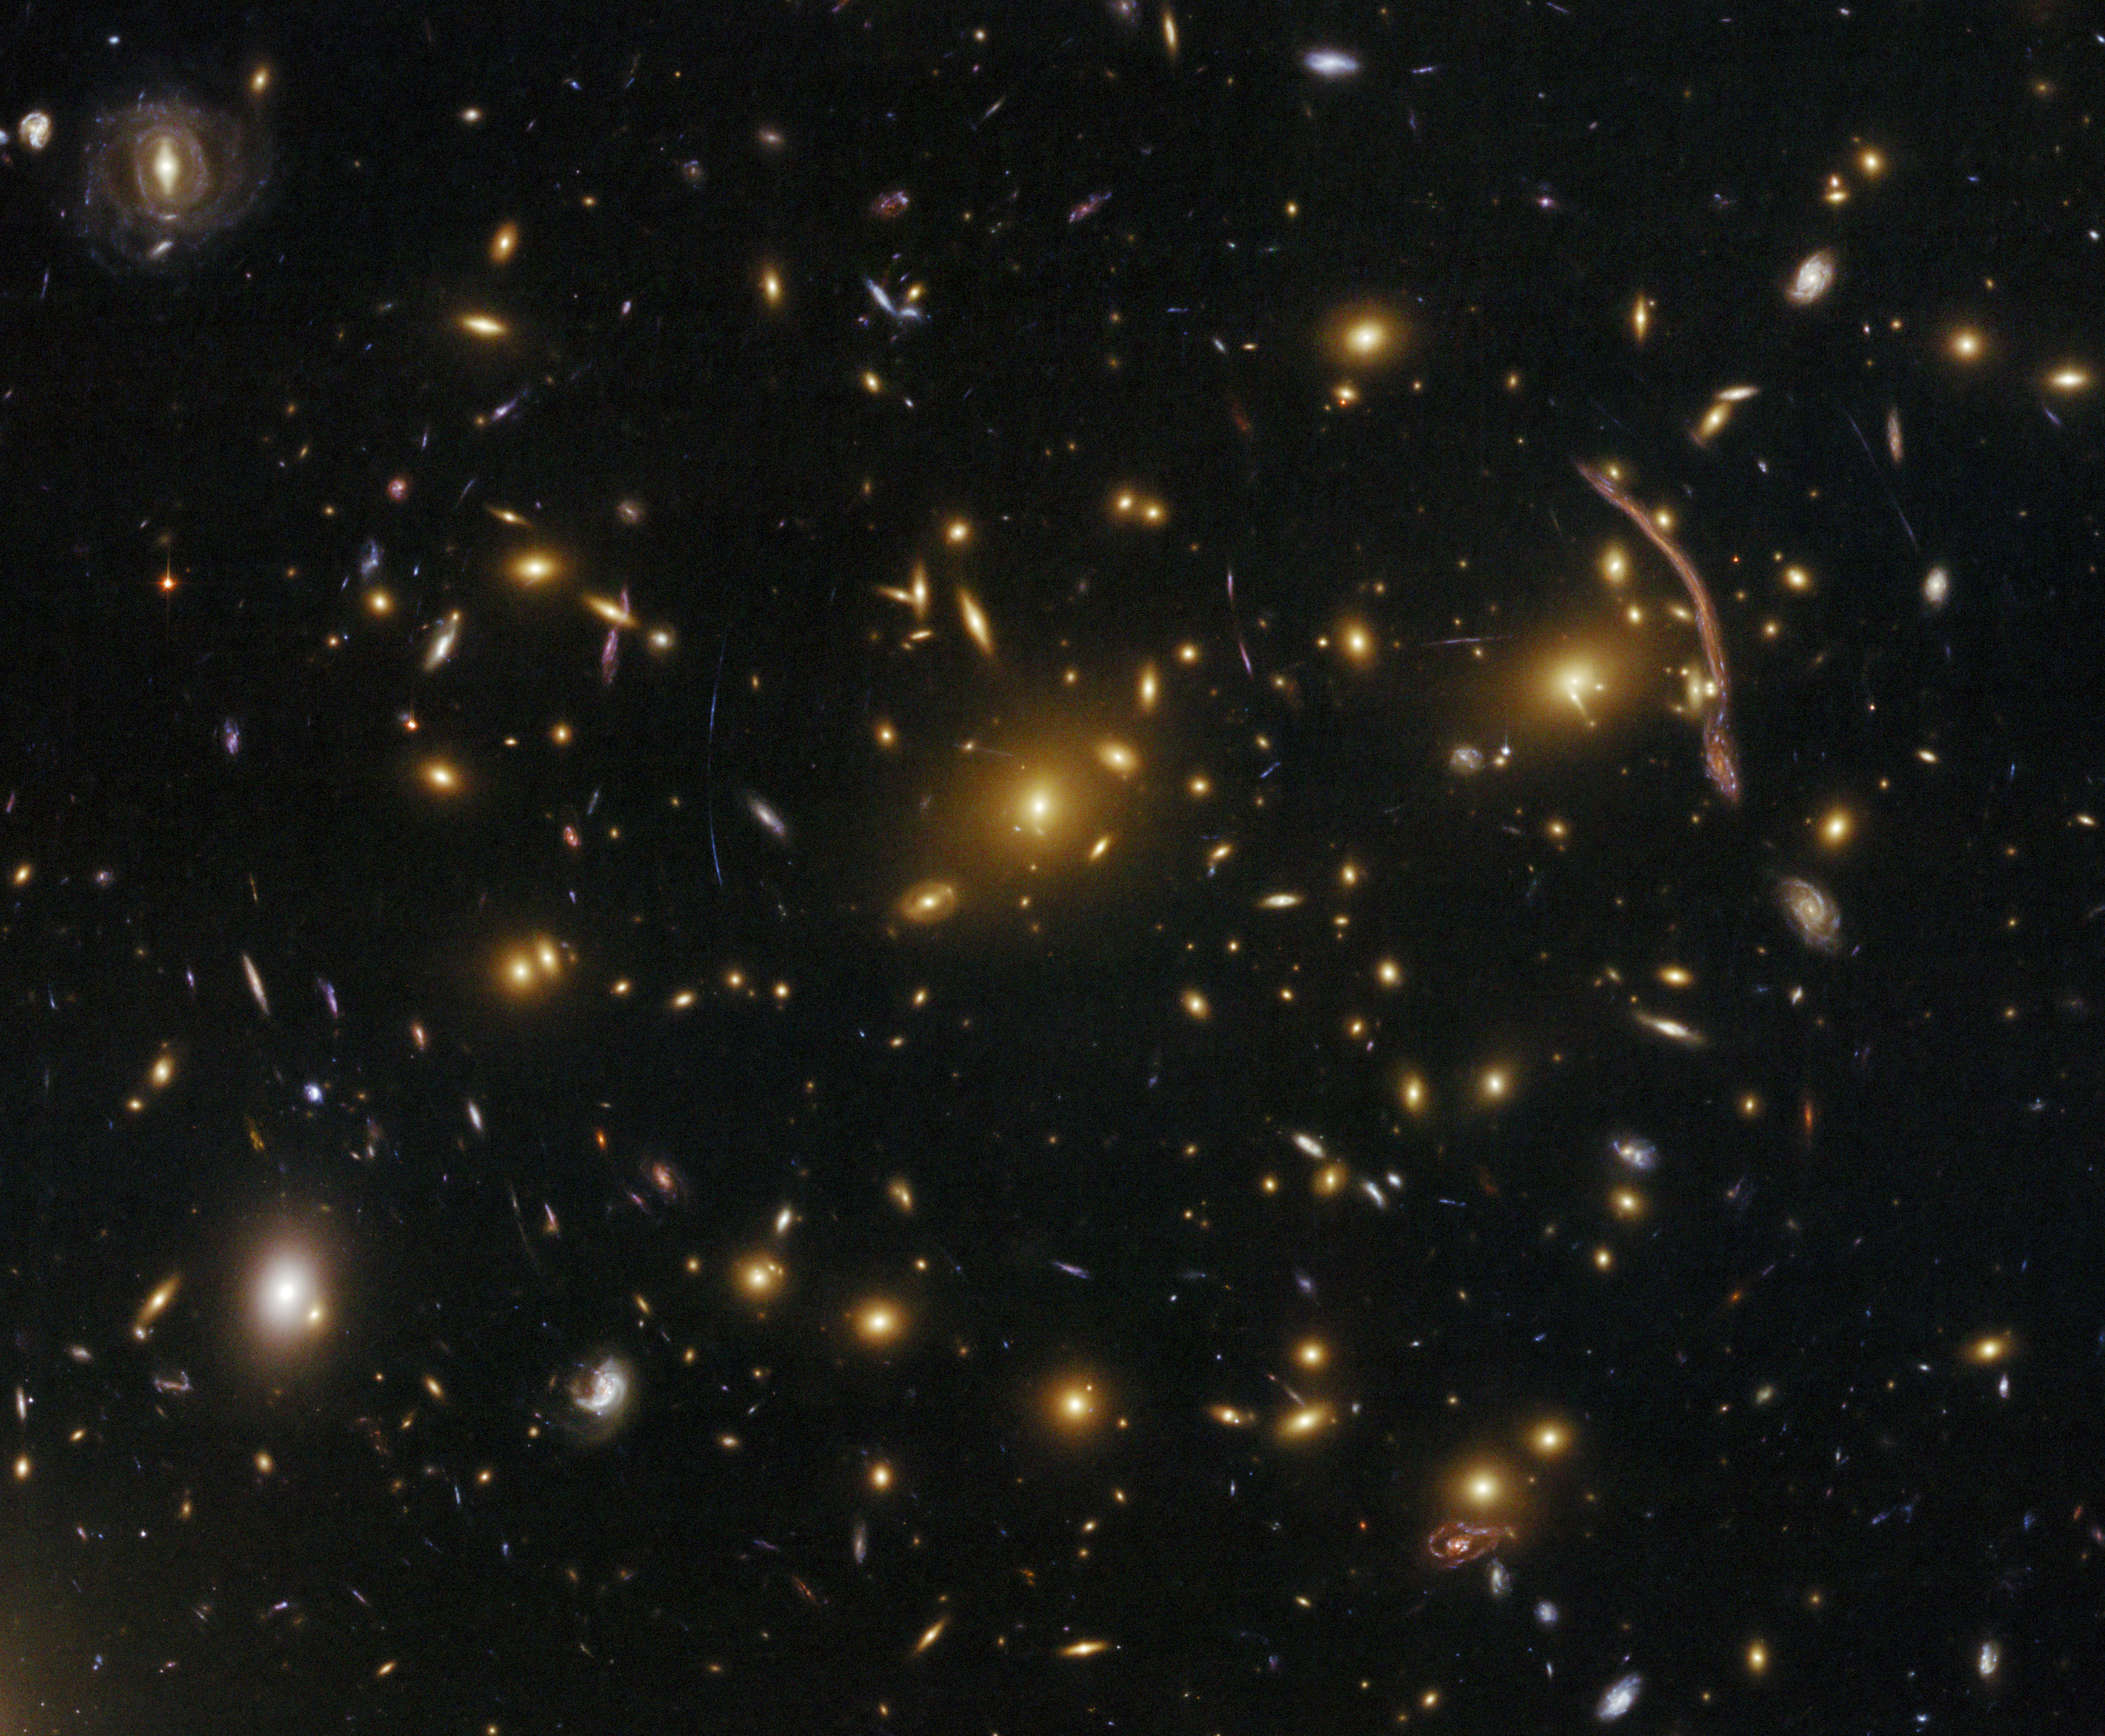
\includegraphics[width=\textwidth]{abell370_hst_med.jpg}
}

\frame{
    \frametitle{Lensing Geometry and Deflection}
    \includegraphics[width=\textwidth]{lens_geometry.pdf}
}

\frame{
    \frametitle{Shear Illustration}
    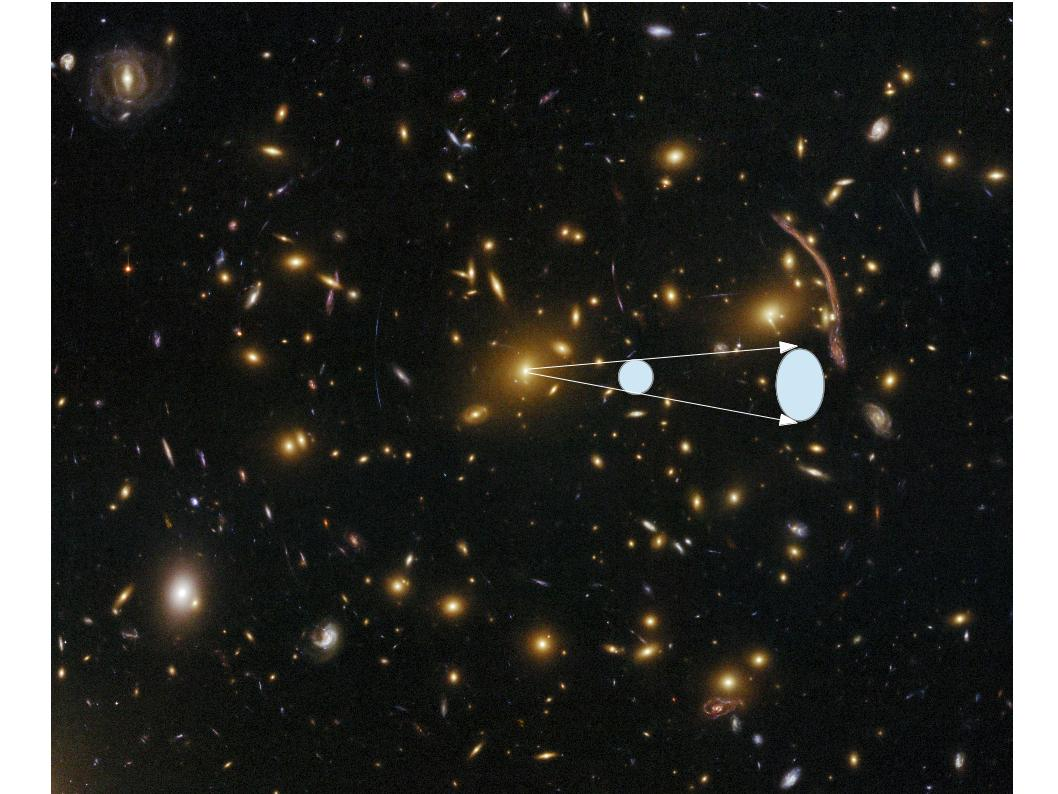
\includegraphics[width=\textwidth]{shear-illustration.jpg}
}

\frame{
    \frametitle{Tangential Shear}
    \begin{columns}
        \begin{column}{0.4\textwidth}
            \fontsize{9}{0.8\baselineskip}
            \begin{itemize}
                \item Tangential Shear
                \item Depends on the projected mass density $\Sigma$.
                \item Depends on the distances to lens and source
            \end{itemize}
        \end{column}
    
        \begin{column}{0.6\textwidth}
            \begin{eqnarray}
                \gamma_{t} & = &  \frac{ \overline{\Sigma}(<R) - \overline{\Sigma}(R)}{ \Sigma_{crit} } \nonumber \\
                           & \equiv &  \frac{\Delta \Sigma}{\Sigma_{crit}} \nonumber \\
                \Sigma_{crit}^{-1} & \propto & D_L \times \frac{ D_{LS} }{D_S} \nonumber
            \end{eqnarray}
        \end{column}
    \end{columns}
}

\frame{
    \frametitle{Cosmology with Lensing}

    \begin{itemize}

        \item Lensing depends on mass and geometry.

        \item If we know where everything is (lens and source) we can use
            lensing to measure mass.

            \begin{itemize}

                \item This is especially useful for measuring the
                    distribution of dark matter in the universe
                \item The connection between galaxies and dark matter.

            \end{itemize}

        \item If we know the mass, or control for it, we can measure geometry.
            
            \begin{itemize}

                \item This is especially interesting for measuring dark energy,
                    which is driving the expansion. 
                \item If we know the redshifts to
                    everything and the absolute distance between everything
                    from lensing, we infer the redshift-distance relation
                    and thus cosmological parameters, including dark energy.

            \end{itemize}

    \end{itemize}
}

\begin{comment}
\frame{
    \frametitle{Ensemble Cluster Lensing}
    
    \begin{itemize}

        \item Clusters are messy and they have neighbors and projected
            structures along the line of sight.

        \item Averaging them together makes the interpretation much simpler.

        \item There is a whopping signal even in the Sloan Digital Sky Survey.

    \end{itemize}
}
\end{comment}

\frame{
    \frametitle{Example: Ensemble Cluster Lensing with SDSS RedMapper}

    Preliminary measurement using SDSS DR8 imaging and the latest RedMapper
    cluster catalog from E. Rykoff.

    \begin{center}
        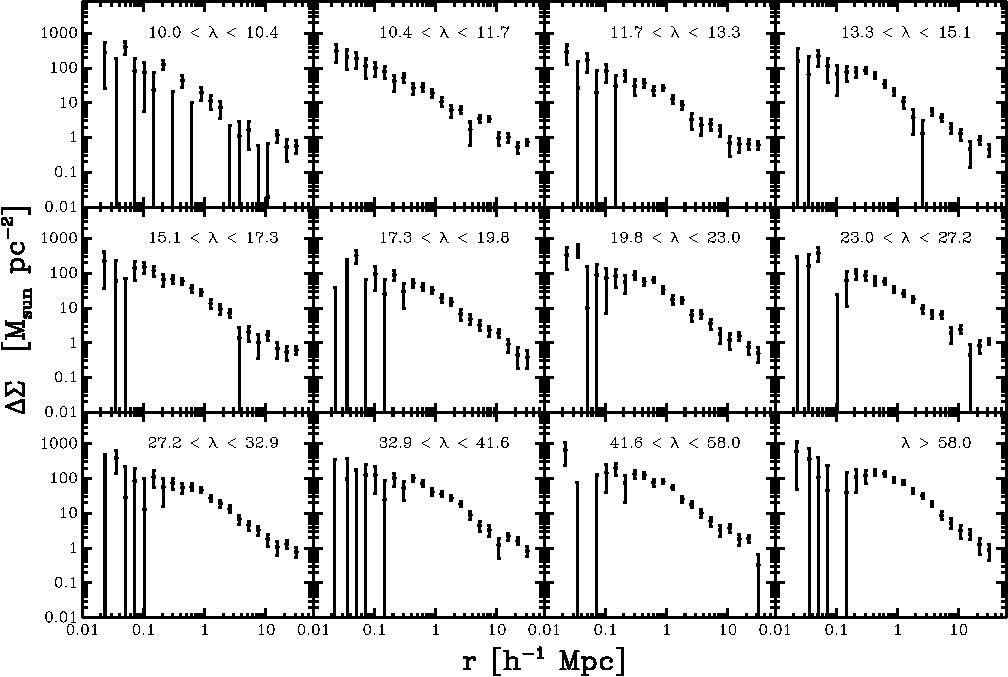
\includegraphics[width=0.8\textwidth]{corrected-rm07s08-lambda-12-allplot.pdf}
    \end{center}
}

\frame{
    \frametitle{Ensemble Cluster Lensing}
    \begin{itemize}

        \item There is tons of $S/N$ even in SDSS, with the Dark Energy Survey
            (DES) the signal will increase because the lenses are at higher
            redshift.

        \item In DES the images are deeper, facilitating using about 10 times more
            galaxies for shear measurement.
         
        \item Precision is great, but how do we know we got the right answer?

    \end{itemize}
}

\frame{
    \frametitle{Did We Get the Right Answer?}

    \begin{itemize}

        \item We might have used the wrong distances.  We don't have redshifts
            for the sources, only 5-filter photometry.  Current and future
            surveys all have this same limitation.

        \item We might have measured the wrong shear.  There are a lot of ways to
            get this wrong: atmosphere, instrument, noise, etc.

    \end{itemize}
}

\frame{
    \frametitle{Photometric Redshifts}
    
    \begin{itemize}
        \item Infer the redshift based on broad band photometry.

        \item Difficult because there are strong degeneracies: e.g. luminous
            blue objects at high redshift look like faint red objects at low
            redshift.

        \item Naive techniques have lots of scatter, significant bias, especially
            as galaxy spectral features move between filters, and a large outlier
            population.

        \item Good progress in recent years with a huge variety of techniques.

    \end{itemize}
}

\frame{
    \frametitle{Ensemble Photometric Redshifts}
    
    \begin{itemize}

        \item Forget about estimating the redshift of a single galaxy
            from the light measured through a few broadband filters. It can't
            be done without strong prior information.

        \item Just try to estimate the overall redshift distribution $N(z)$.

        \item For much lensing work $N(z)$ is sufficient.
        
        \item Secondarily try to learn something about the probability distribution
            as a function of redshift for each galaxy $P(z)$.  Useful as a weight
            for studies such as ensemble cluster lensing.

    \end{itemize}
}

\frame{
    \frametitle{Ensemble Photometric Redshifts}
    
    \fontsize{10}{0.8\baselineskip}
    \begin{itemize}

         \item Hypothesis: If the distribution of all relevant observables are
             the same for two populations then so are the redshift distributions
             $N(z)$.

         \item Find a set of weights such that the distribution of observables
             for training set galaxies with spectroscopic redshifts matches the
             observables for a set of galaxies without redshifts.  Then the
             weighted redshift histogram will also match, and that is an
             estimate of $N(z)$.

         \item Can break down if the two samples have very different selection
             in a redshift-correlated variable that is accounted for, but it
             turns out this is not a dominant problem in practice (Cunha et al.
             2012).


         \item \texttt{ProbWTS}: Probability Distributions
             from Weight Training Sets. References: Lima et al. 2008, Cunha et al.
             2008, Sheldon et al. 2012.

    \end{itemize}

}


\frame{
    \frametitle{Weighting Method: Tests on DES Mocks}

    \begin{columns}

        \begin{column}{0.4\textwidth}
            \begin{itemize}

                \item DES Mock catalogs

                \item with very different magnitude
                    distributions for spectroscopic training sample and
                    photometric only sample.

            \end{itemize}
        \end{column}

        \begin{column}{0.6\textwidth}

            \begin{center}
                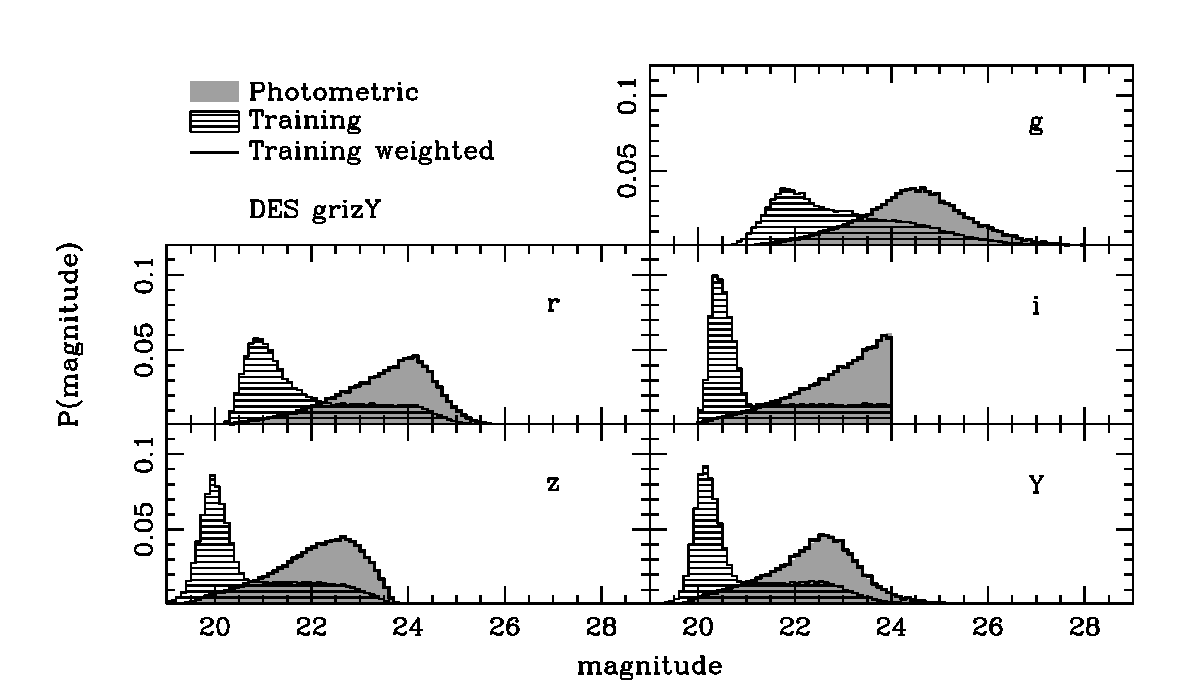
\includegraphics[width=\textwidth]{lima-fig4-maghist.pdf}
                \newline
                Lima et al. 2008
            \end{center}

        \end{column}

    \end{columns}


}

\frame{
    \frametitle{Weighting Method: Tests on DES Mocks}

    \begin{columns}

        \begin{column}{0.5\textwidth}
            \begin{itemize}

                \item Training set very different magnitudes and
                    redshift distribution.

                \item Good recovery of underlying $N(z)$.

                \item Uncertainties are dominated by sample variance
                    (Cunha et al. 2012)


            \end{itemize}
        \end{column}

        \begin{column}{0.5\textwidth}

            \begin{center}
                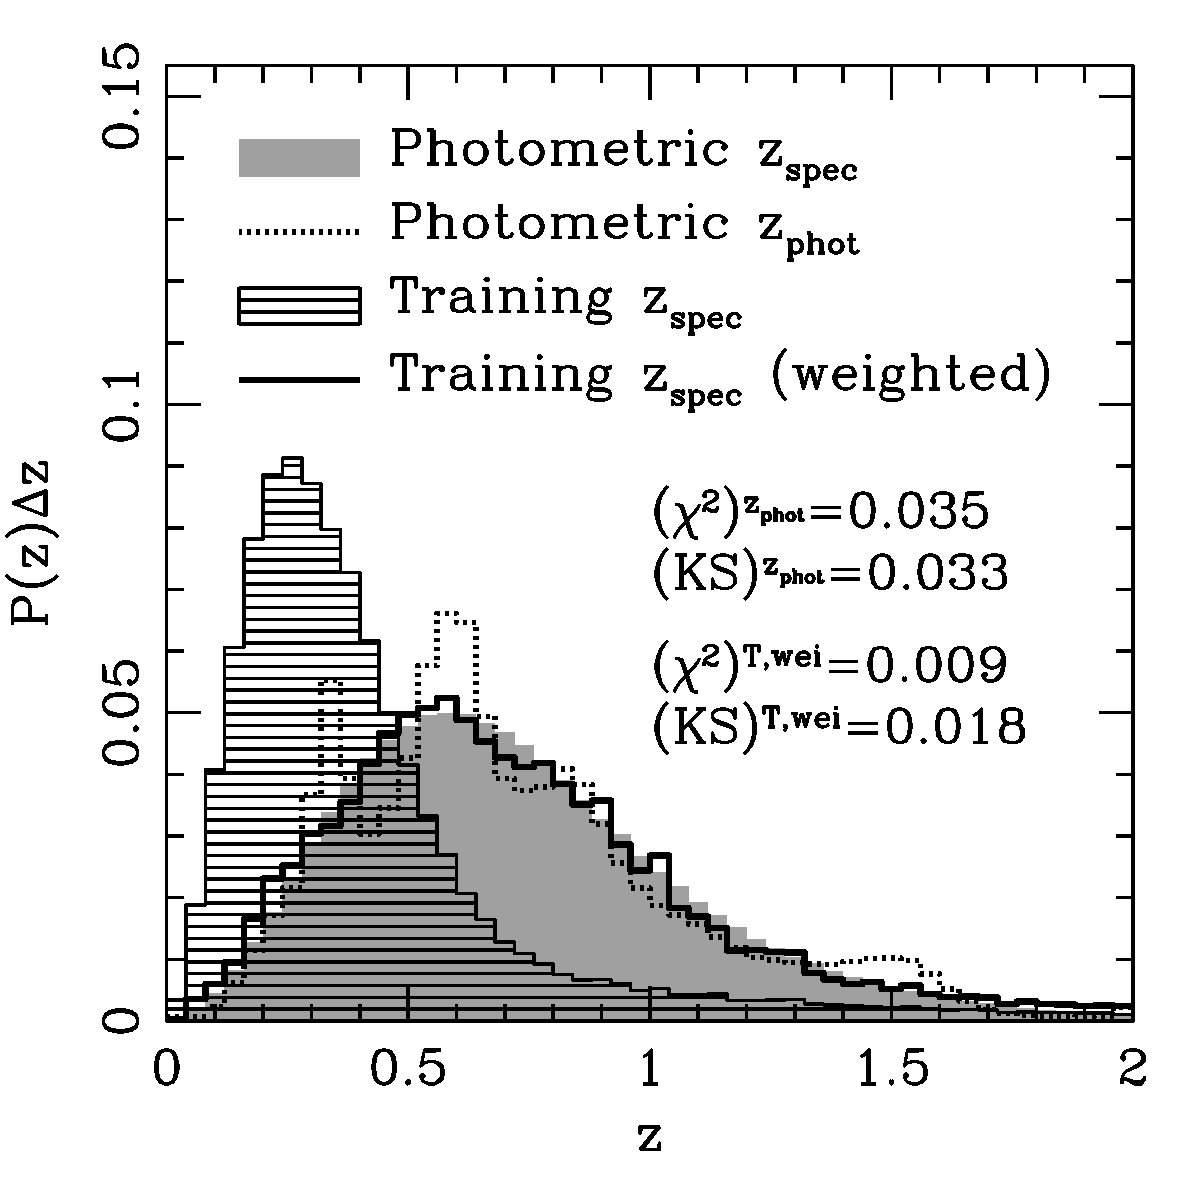
\includegraphics[width=\textwidth]{lima-fig5-recovery.pdf}
                \newline
                Lima et al. 2008
            \end{center}

        \end{column}

    \end{columns}
}

\frame{
    \frametitle{Weighting Method: Application to SDSS Data}

    \begin{columns}

        \begin{column}{0.5\textwidth}
            \begin{center}
                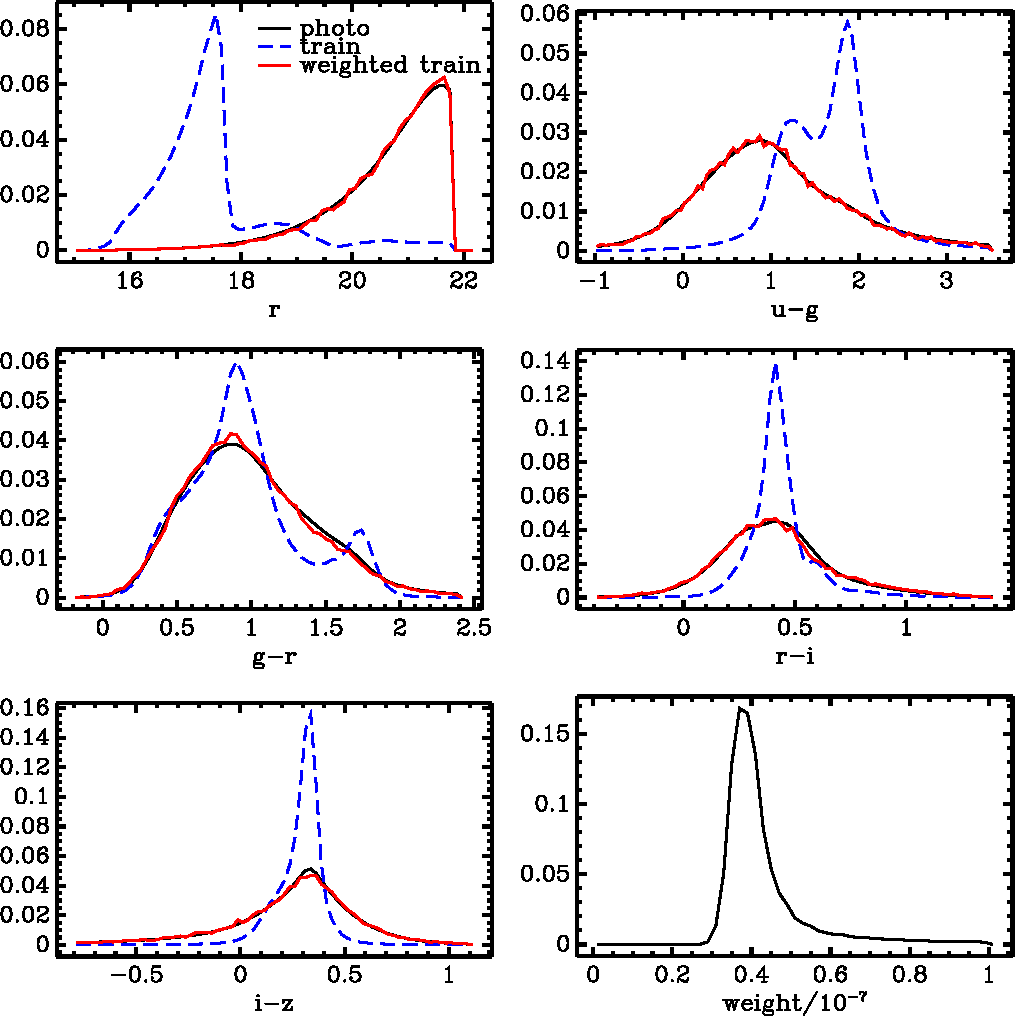
\includegraphics[width=\textwidth]{zweight-10-varhist.pdf}
            \end{center}
        \end{column}

        \begin{column}{0.5\textwidth}
            \begin{center}
                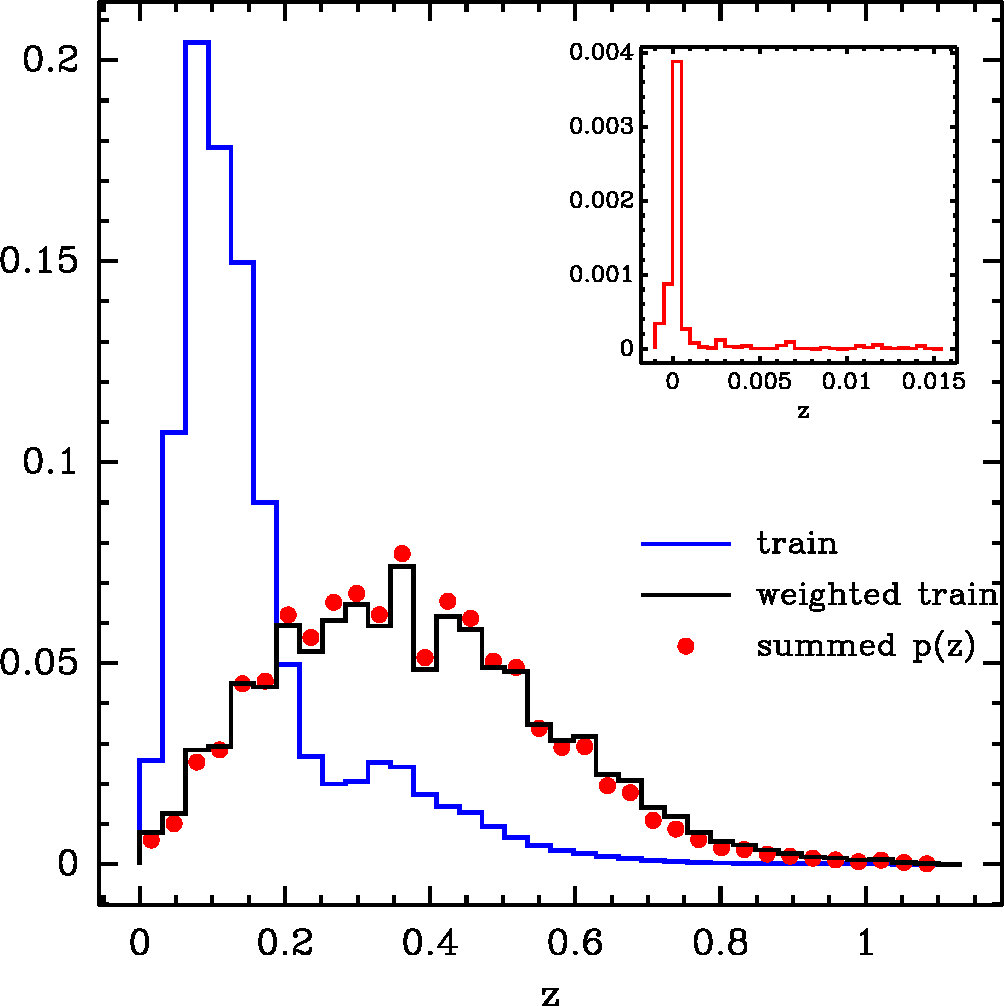
\includegraphics[width=\textwidth]{zweight-10-zhist-withorig-withsum-12.pdf}
                \newline
                Sheldon et al. 2008
            \end{center}
        \end{column}


    \end{columns}

}

\frame{
    \frametitle{What Does This Mean for Lensing Measurements?}

        Systematic errors in $N(z)$ translate into a calibration error
        for the shear.

    \begin{center}
        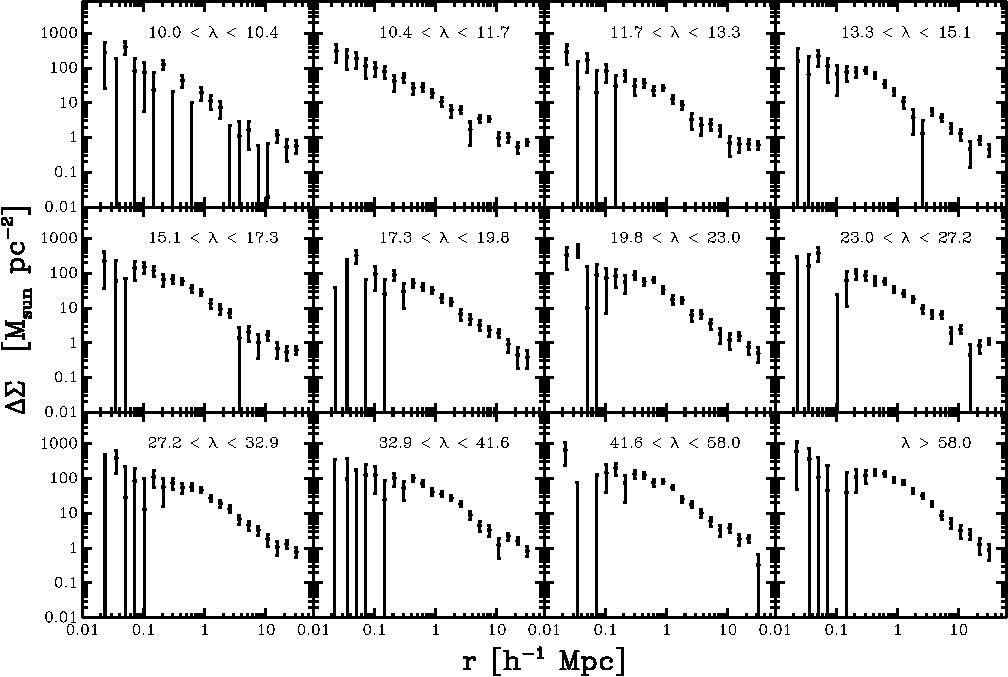
\includegraphics[width=0.8\textwidth]{corrected-rm07s08-lambda-12-allplot.pdf}
        \newline
        Preliminary
    \end{center}
}



\frame{
    \frametitle{Weighting Method: Expected Lensing Bias}

    \fontsize{9}{0.8\baselineskip}
    \begin{columns}

        \begin{column}{0.5\textwidth}
            \begin{itemize}


                \item Any systematic error in $N(z)$ translates to an error in
                    distance and thus errors in the measured mass.
                
                \item Using a subset of the SDSS sample with redshifts in DEEP
                    as validation shows the weighting method works well for
                    lenses in the redshift range of interest $\left[0.0,
                    0.3\right]$.

                \item For DES we need this to work for lens redshifts near
                    unity.  Calculations indicate it can work as long as we
                    have less than a percent of wrong redshifts in training
                    sample.  (Cunha et al. 2012)


            \end{itemize}
        \end{column}

        \begin{column}{0.5\textwidth}

            \begin{center}
                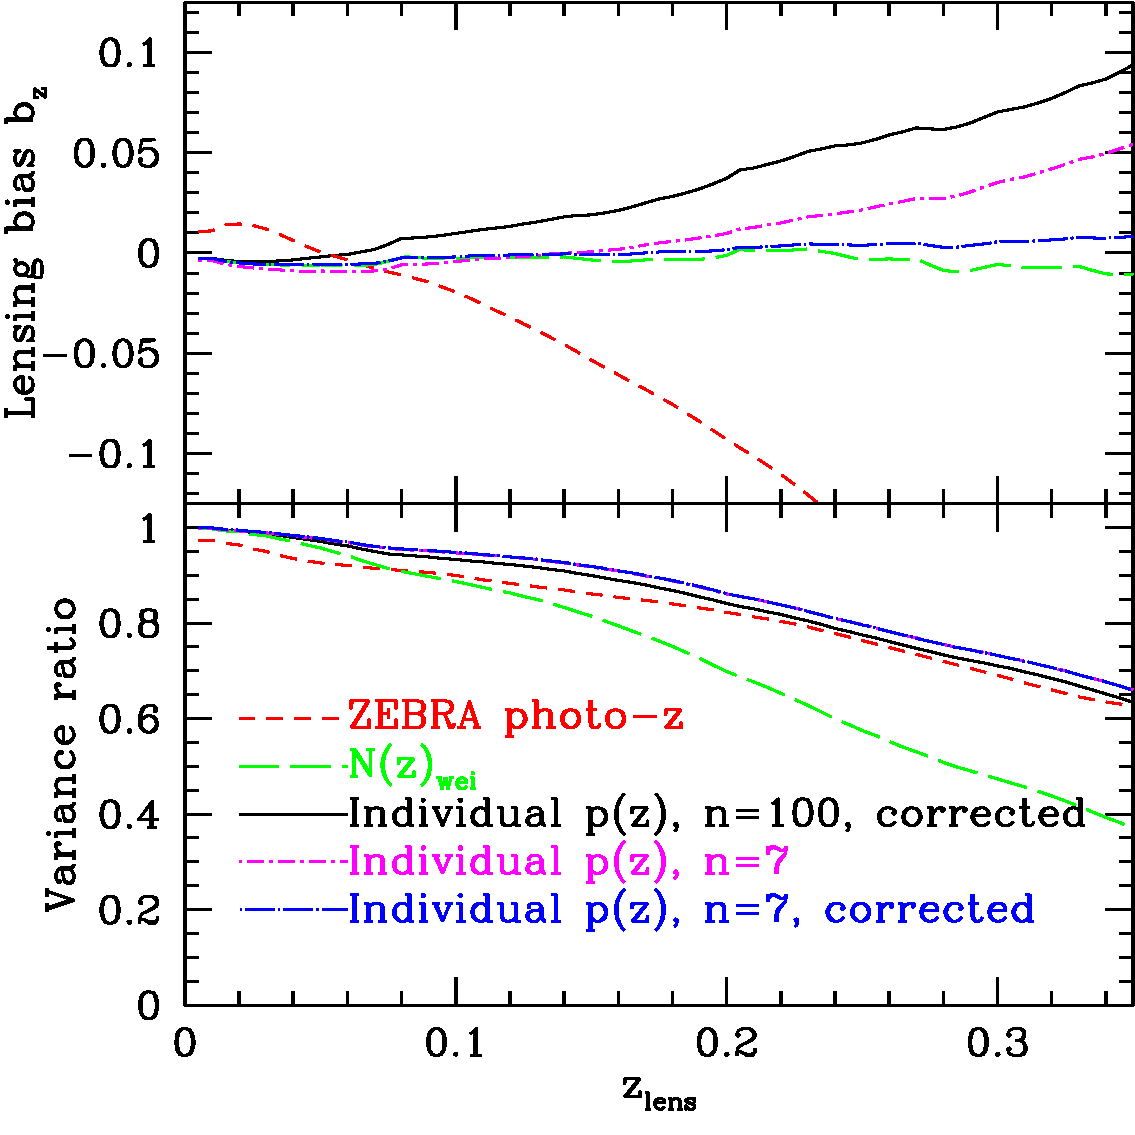
\includegraphics[width=\textwidth]{pz-egs-c3n7-paper.pdf}
                \newline
                Sheldon et al. 2012
            \end{center}

        \end{column}

    \end{columns}
}

\frame{
    \frametitle{Shear Estimation}
    \begin{center}
        Sources of error in shear measurement.
        \newline

        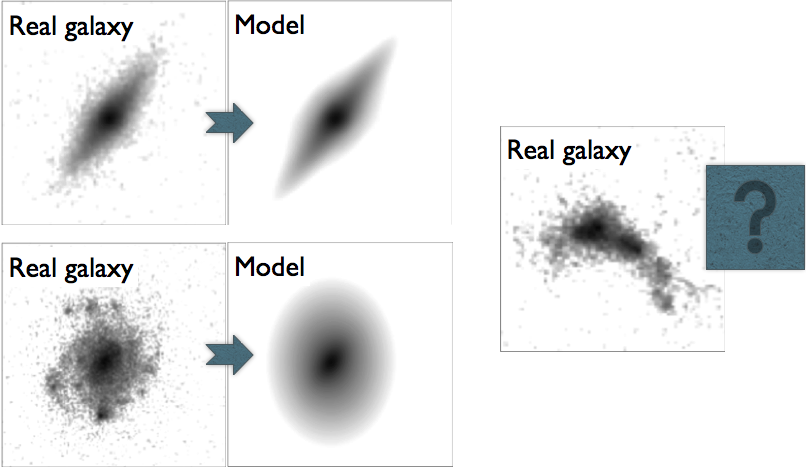
\includegraphics[width=0.7\textwidth]{real_gal.png}
        \newline

        {\scriptsize Mandelbaum. et al. Great 3 Handbook}

    \end{center}
}

\frame{
    \frametitle{Shear Estimation}

    Sources of error in shear measurement.
    \newline

    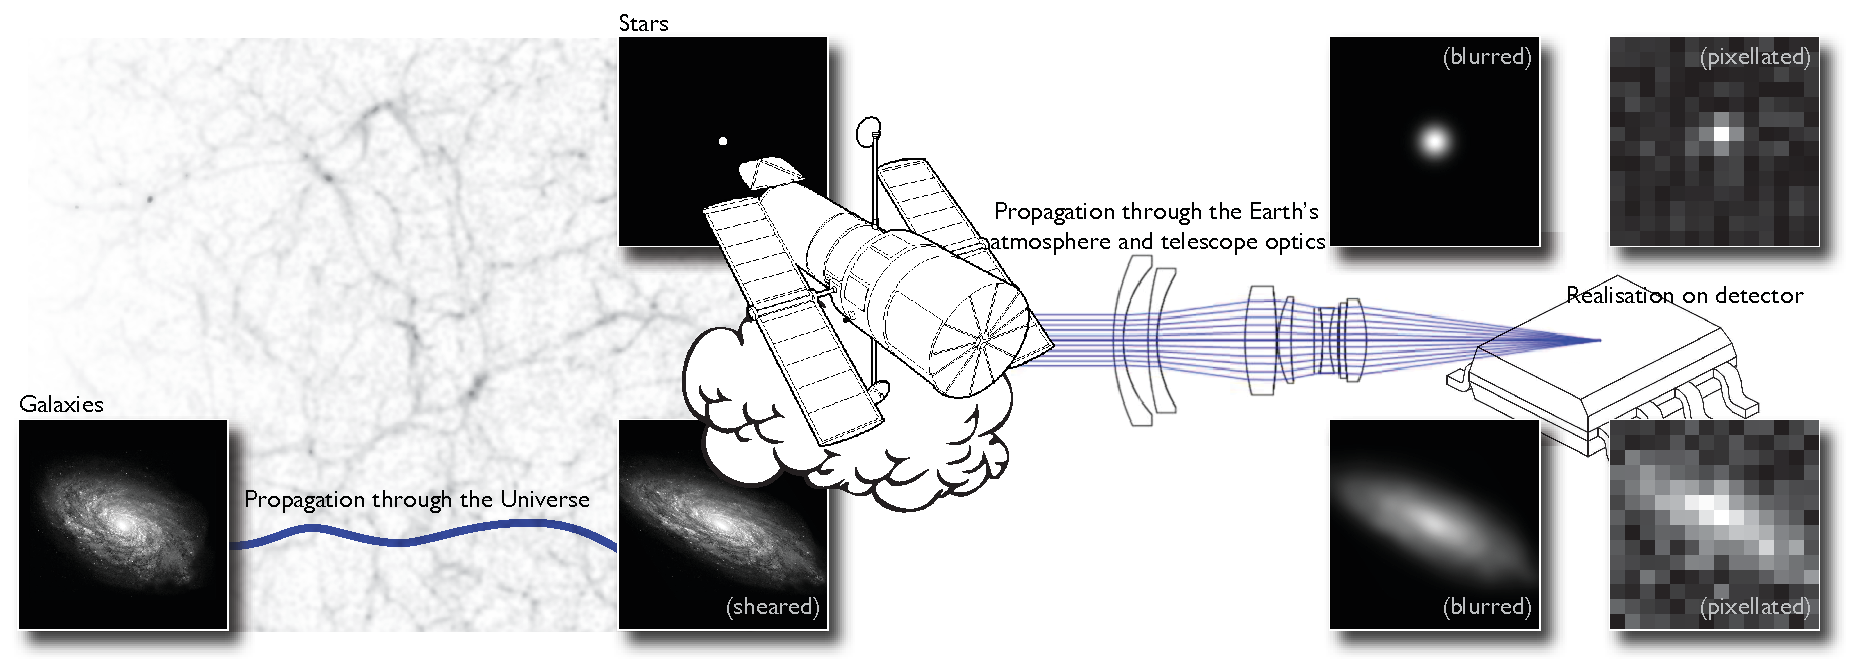
\includegraphics[width=\textwidth]{forward_G3.pdf}
    \newline
    {\scriptsize Mandelbaum. et al. Great 3 Handbook}
}


\frame{
    \frametitle{Noise}

    \begin{itemize}

        \item For low $S/N$ galaxy images, naive techniques to measure shear
            from a galaxy ellipticity break down and this dominates the
            systematic error.

        \item Non-linear fitting in the presence of noise is biased, both the
            maximum likelihood and expectation value: using the mean shape
            won't work (Hirata, Refregier, etc).   Results in a {\bf
            calibration} error.

        \item Weighted moments can alleviate the problem somewhat, but there
            can still be of order 10\% errors at $S/N=10$.

        \item This is generally known in statistics, but not recognized for our
            particular problem until relatively recently. Badly aggravated by
            the PSF ``deconvolution''.


    \end{itemize}
}

\frame{
    \frametitle{Extreme Example: Noise Bias using the Expectation Value}
    \begin{center}

        \includegraphics[width=0.7\textwidth]{cbafit-geg07-geg08-deg03-deg05-gmean-flux-s2n.pdf}
        \newline

    \end{center}
}



\frame{
    \frametitle{Ensemble Shear Measurement}
    
    \begin{itemize}

        \item Bernstein \& Armstrong 2014

        \item Forget about estimating a weak shear from a single galaxy
            image. It can't be done.  Galaxies are elliptical and this
            noise dominates, so you have to average anyway.

        \item But we know true things that can help: the posterior
            distribution of the mean shear averaged from many galaxies must
            approach a Gaussian: central limit theorem.
        
        \item We also know the shear is weak.

        \item Assuming Gaussianity, weak shear, and knowledge of underlying
             distribution of shapes for the ensemble (the prior), one can
             derive an unbiased estimator for the mean shear of the ensemble.


    \end{itemize}
}


\frame
{
    \frametitle{Bernstein \& Armstrong}

    \fontsize{8}{0.8\baselineskip}

    Assume a small shear \vecg.  The posterior probability for
    the shear estimated from many galaxies is

    \begin{eqnarray}
    P(\vecg | {\bf D}) & = & \frac{ P(\vecg) P({\bf D}|\vecg ) }{ P({\bf D}) }  \\
                        & = & P(\vecg) \prod_i \frac{ P({\bf D}_i | \vecg) }{ P({\bf D}_i) } \\
        P({\bf D}_i | \vecg) & \approx & P_i + \vecg  \cdot \vecQ_i + \frac{1}{2} \vecg \cdot \matR_i \cdot \vecg \\
        -\textrm{ln} P(\vecg | {\bf D}) & \approx & (\textrm{stuff})  - 
        \vecg \cdot \sum_i \frac{ \vecQ_i }{P_i} + \frac{1}{2} \vecg \cdot \left[ \sum_i \left( \frac{ \vecQ_i \vecQ_i^T}{P_i^2} - \frac{ \matR_i }{P_i} \right) \right] \cdot \vecg
    \end{eqnarray}
    
    Note the \vecQ\ and \matR\ involve first and second derivatives of the
    prior (the true shape distribution) with respect to shear. In practice the
    \vecQ\ and \matR\ are averaged over the likelihood surface.

}

\frame
{
    \frametitle{Bernstein \& Armstrong}

    Then the shear can be solved for directly

    \begin{eqnarray}
    \matC_g^{-1} & = & \sum_i \left(\frac{\vecQ_i \vecQ^T_i}{P_i^2} - \frac{\matR_i}{P_i}\right) \label{eq:cdef} \nonumber \\
    \bar{\vecg} & = &  \matC_g \sum_i \frac{\vecQ_i}{P_i}. \label{eq:shdef}
    \end{eqnarray}

}

\frame{
    \frametitle{Bernstein \& Armstrong}

    \fontsize{10}{0.8\baselineskip}
    \begin{itemize}

        \item Bernstein \& Armstrong gave a simple demonstration but no
            implemenation to work with images.

        \item Computationally challenging to measure the full likelihood
            surface in a high dimensional space.
            
        \item Even the fastest existing codes took seconds to perform a few
            hundred likelihood evaluations.  Tens of thousands are needed here.

        \item My solution is to make lots of approximations:  use Gaussian
            mixtures for the galaxy models (Hogg and Lang 2013) and the PSF.
            Then the convolutions are fast and analytic. Use a fast approximate
            exponential function, etc.

        \item Can perform a likelihood evaluation in 100 microseconds,
            search the full space in a few seconds.

        \item Just submitted to the arXiv over the weekend (Sheldon 2014)

    \end{itemize}
}


\frame{
    \frametitle{Bayesian Shear Estimation: Test By Simulation}

    \fontsize{9}{0.8\baselineskip}
    \begin{columns}

        \begin{column}{0.5\textwidth}
            \begin{itemize}

                \item Simulate galaxies with \sersic\ index $n=1$ for
                    exponential radial profile (like spiral galaxies) and $n=4$
                    for \devauc\ profile (like early type galaxies).

                \item PSF-convolved size just bigger than the PSF, similar to
                    what you get from star-galaxy separation for faint noisy
                    galaxies.

                \item In these controlled conditions, sufficiently
                    unbiased for current surveys (light gray) and future
                    surveys (dark gray).

                \item No other published method meets these requirements
                    without some kind of post-calibration based
                    on simulations.

            \end{itemize}
        \end{column}

        \begin{column}{0.5\textwidth}

            \begin{center}
                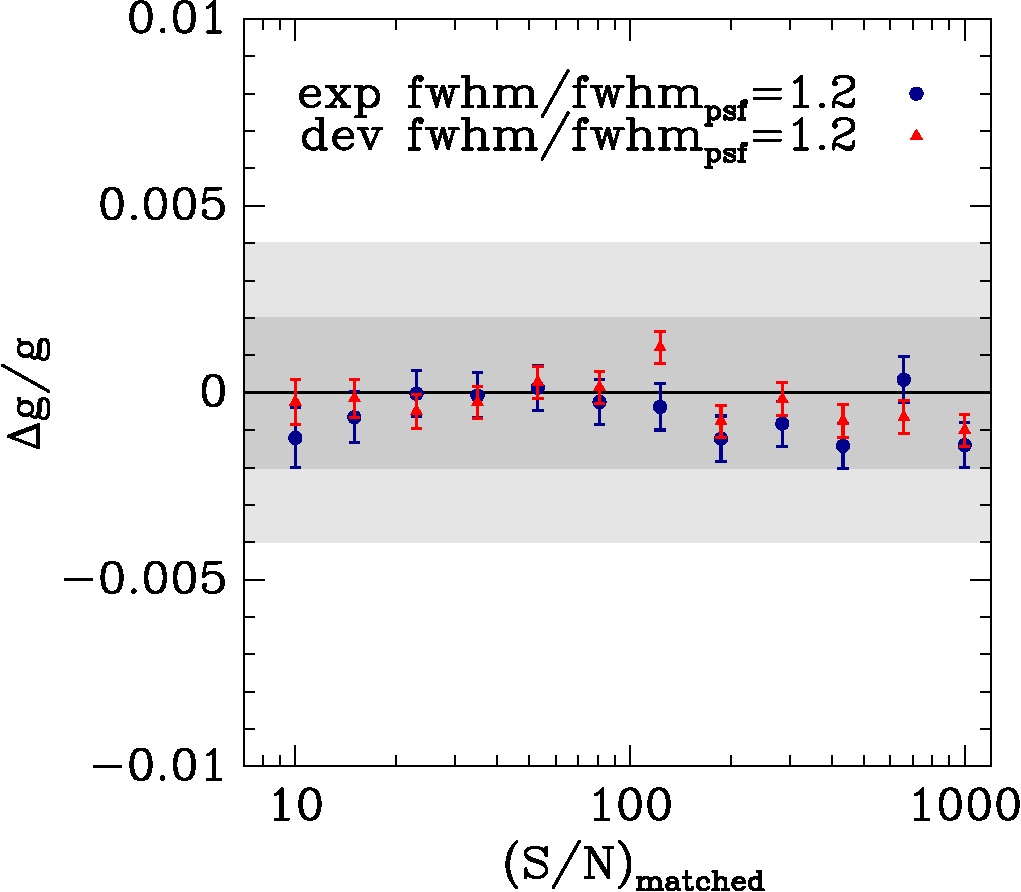
\includegraphics[width=\textwidth]{ngmix-fwhm1_2.pdf}
                \newline
                Sheldon 2014
            \end{center}

        \end{column}

    \end{columns}
}



\begin{comment}

\frame{

    \frametitle{Gravitational Shear}

    \fontsize{10}{0.8\baselineskip}

    \begin{columns}

        \begin{column}{0.5\textwidth}

            \begin{itemize}
                \item The path of light appears curved as it passes massive objects
                \item The ``deflection'' can differ across the face of an extended source galaxy, causing distortion.
                \item Shear distorts the image; we say it's ``shape'' is altered.
                \item For small shears, a circle becomes a pure ellipse.
                \item Shearing produces correlations in the shapes of galaxies across the sky.
                    Shape correlations are closely related to mass density
                    correlations.

            \end{itemize}
        \end{column}
        \begin{column}{0.5\textwidth}
            \includegraphics[width=\textwidth]{shear-illustration-crop.jpg}
            \newline
            \begin{center}
                {\small Note galaxies aren't round!  ``Shape noise''}
            \end{center}
        \end{column}
    \end{columns}
}

\frame{
    \frametitle{Shear}
    \fontsize{10}{0.8\baselineskip}

    \begin{columns}
        \begin{column}{0.5\textwidth}
            \begin{itemize}

                \item The correlations in the shear/matter field hold a lot of
                    information about the {\bf Dark Matter} distribution.  The Cold Dark
                    Matter theory predicts these correlations.

                \item Shear depends on the distances to the lens and source. The
                    distance dependence encodes the expansion rate of the universe and
                    thus {\bf Dark Energy}.

                \item To meet goals of current surveys we want to measure shear to
                    about 0.3-0.4\% accuracy (e.g.  Dark Energy Survey).  LSST about
                    a factor of five better.

            \end{itemize}
        \end{column}

        \begin{column}{0.5\textwidth}
            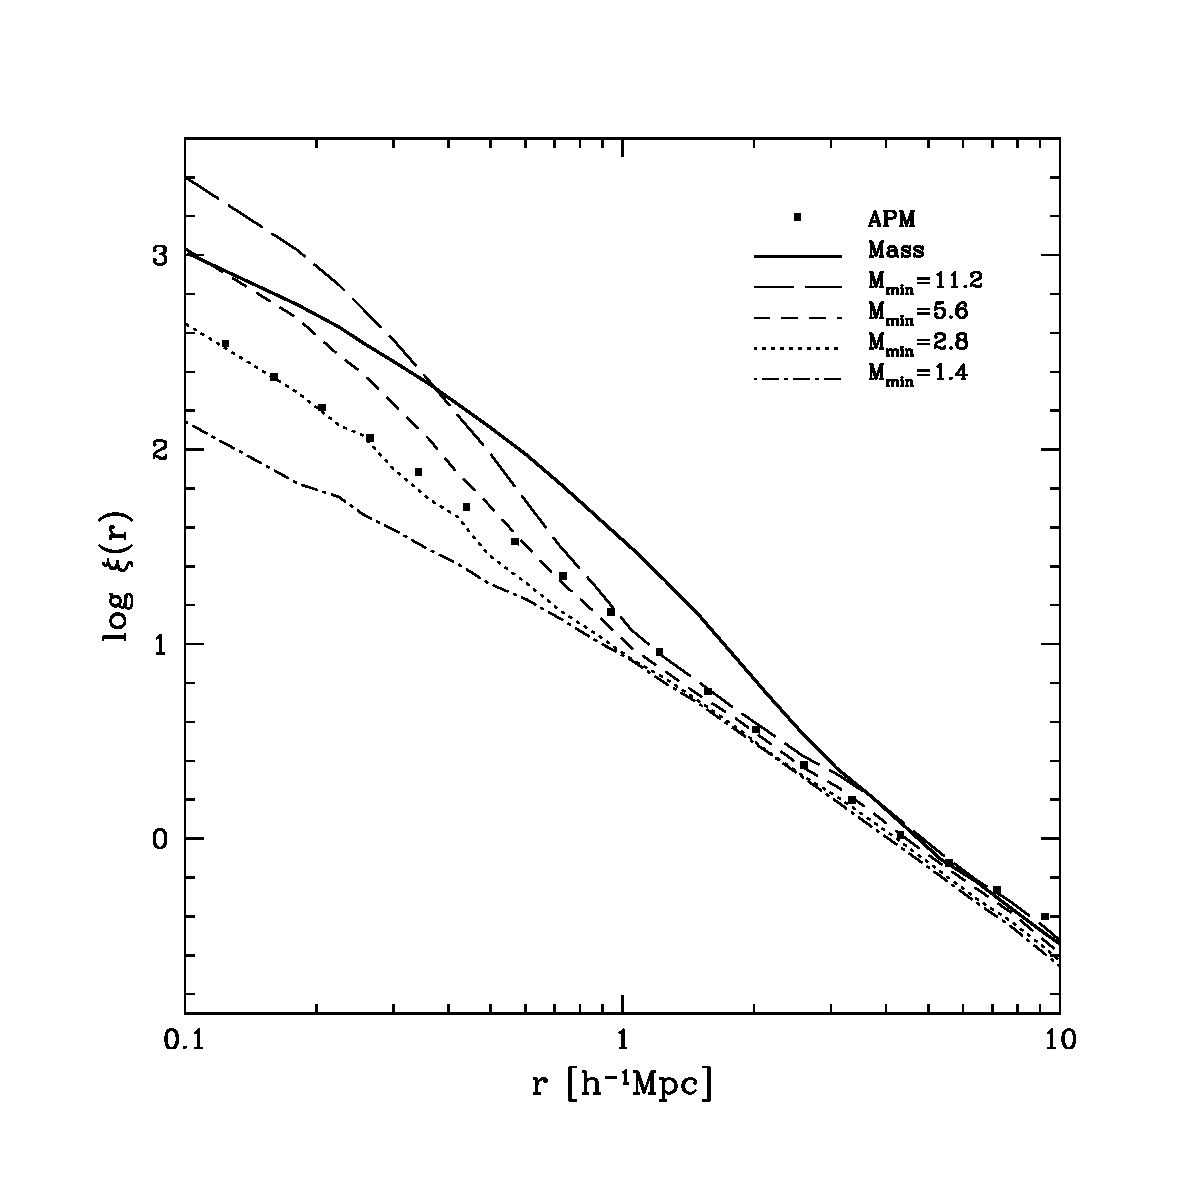
\includegraphics[width=\textwidth]{berlind-weinberg-f3.pdf}
            \newline
            \begin{center}
                {\tiny Berlind \& Weinberg 2002}
            \end{center}
        \end{column}
    \end{columns}
}



\frame{
    \frametitle{Measuring Shear}

    \begin{itemize}
        \item For a perfect detector with no noise, just measure
            the second moments and look for the correlations.
        \item ... but the atmosphere, telescope, and instrument smear
            the image: the Point Spread Function (PSF).
        \item Convolution just adds to the moments, so we just need to
            subtract off the PSF moments!

        \item ... but there is noise, so error in moments blows up (among other
            difficulties).

    \end{itemize}
}

\frame{
    \frametitle{PSF and Noise}
    
    \begin{itemize}

        \item One can use a weight function to suppress the noise, but then one
            must derive how that measurement responds to smearing by the PSF
            and shearing (e.g. Kaiser, Squires, \& Broadhurst, Bernstein \& Jarvis, Melchior,
                    Bernstein \& Armstrong).  Working in Fourier space can help
            with the deconvolution (Bernstein).

        \item Alternatively, one can forward-model the problem: fit a model that is
            convolved with an estimate of the PSF.  Limited by how well one can
            model the galaxy and PSF (e.g. Miller et al., Bernstein \& Armstrong, many
            others).

        \item These methods can be made to work well, as long as the $S/N$ is
            still pretty high, say 50 or higher.

    \end{itemize}
}

\frame{
    \frametitle{Noise}

    \begin{itemize}
        \item When the $S/N$ is low, these techniques break down.

        \item Non-linear fitting in the presence of noise is biased, both the
            maximum likelihood and expectation value: using the mean shape
            won't work (Hirata, Refregier, etc).   Results in a {\bf
            calibration} error.

        \item This is generally known in statistics, but not yet solved
            for our particular problem. Badly aggravated by the PSF ``deconvolution''.
        \item The noise also causes problems for moment based methods.
    \end{itemize}
}

\frame{
    \frametitle{Maximum Likelihood}

    \begin{center}
    \includegraphics[width=0.7\textwidth]{{gmix-fit-gg05r01-yr-0.005-0.005-diff}.pdf}
\end{center}

}

%\section{Bayesian Methods}

\frame{
    \frametitle{Miller et al. 2007}

    \begin{itemize}

        \item Miller et al. 2007 (LENSFIT): Use priors on the parameters and
            explore a constrained posterior surface (Prior $\times$
            Likelihood).

        \item Attempt to derive how the shear estimate (the shape) affected by
            the noise and prior using integrals over the posterior surface and
            first order approximation in shear.  Called the {\bf response}.

        \item The posterior surface of the shape for a single galaxy is
            complex.  The space is bounded, the surface is necessarily
            asymmetric and depends on galaxy properties and noise.

        \item No rigorous expression is given for the mean shear of a
            population given these ellipticity responses.  Choose to simply
            average them.

        \item Miller et al. 2013 find large biases in simulations, of
            order 10\% at \snflux$ \sim 10$.
        
    \end{itemize}
}

\frame{
    \frametitle{LENSFIT Tests}

    \begin{columns}
        
        \begin{column}{0.5\textwidth}
            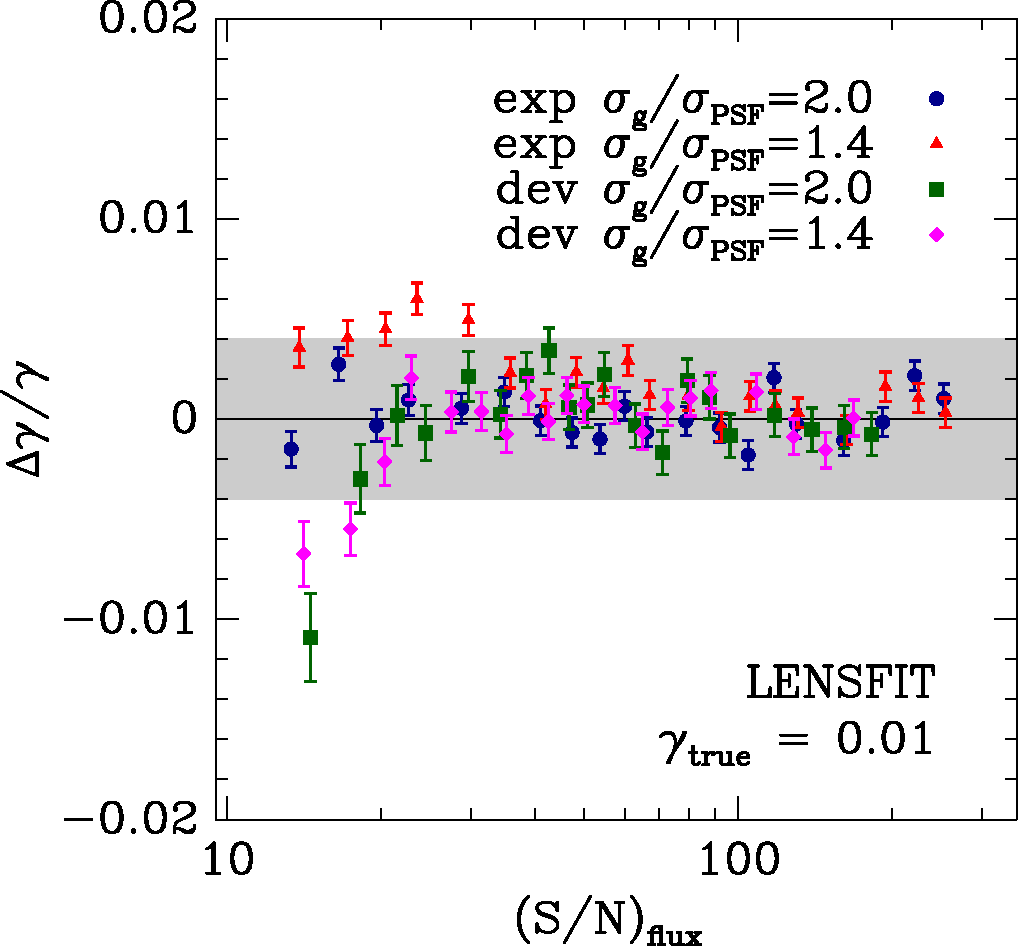
\includegraphics[width=\textwidth]{cbafit-geg07-geg08-deg03-deg05-lensfit-flux-s2n.pdf}
        \end{column}

        \begin{column}{0.5\textwidth}
            \includegraphics[width=\textwidth]{cbafit-geg07-geg08-deg03-deg05-lensfit-T-s2n.pdf}
        \end{column}
    \end{columns}

    \fontsize{9}{0.8\baselineskip}
    \begin{itemize}
        \item I did my own tests of LENSFIT with strong structural priors (30\% lognormal
            on flux, 15\% on size (that was a bug...) ).

        \item Very fast code using gaussian mixtures to approximate galaxies.  Fast
            analytic convolutions.

        \item Bias vs \snT\ has more universal form than vs \snflux.
    \end{itemize}

}

\frame{
    \frametitle{Bernstein \& Armstrong 2013}

    \begin{itemize}

        \item Shape is not shear.
        \item While the posterior surface for the {\it shape} of single galaxy
            is complex, the posterior surface for the {\it mean shear} of an
            ensemble must approach a Gaussian according to the central limit
            theorem.  This is both useful and actually true!

         \item Assuming Gaussianity, weak shear, and knowledge of underlying
             distribution of shapes for the ensemble (the prior), one can
             derive an unbiased estimator for the mean shear of the ensemble.

         \item You lose nothing: in the limit of weak shear, you need
             to use an ensemble statistic anyway.  The ``shape noise'',
             intrinsic variance in shapes of galaxies, dominates over
             the signal.

        \item This is a good idea, but needed an implementation, so I worked it
            into my existing code.
         
    \end{itemize}

}

\frame{
    \frametitle{BA13 Tests}

    \begin{columns}
        
        \begin{column}{0.5\textwidth}
            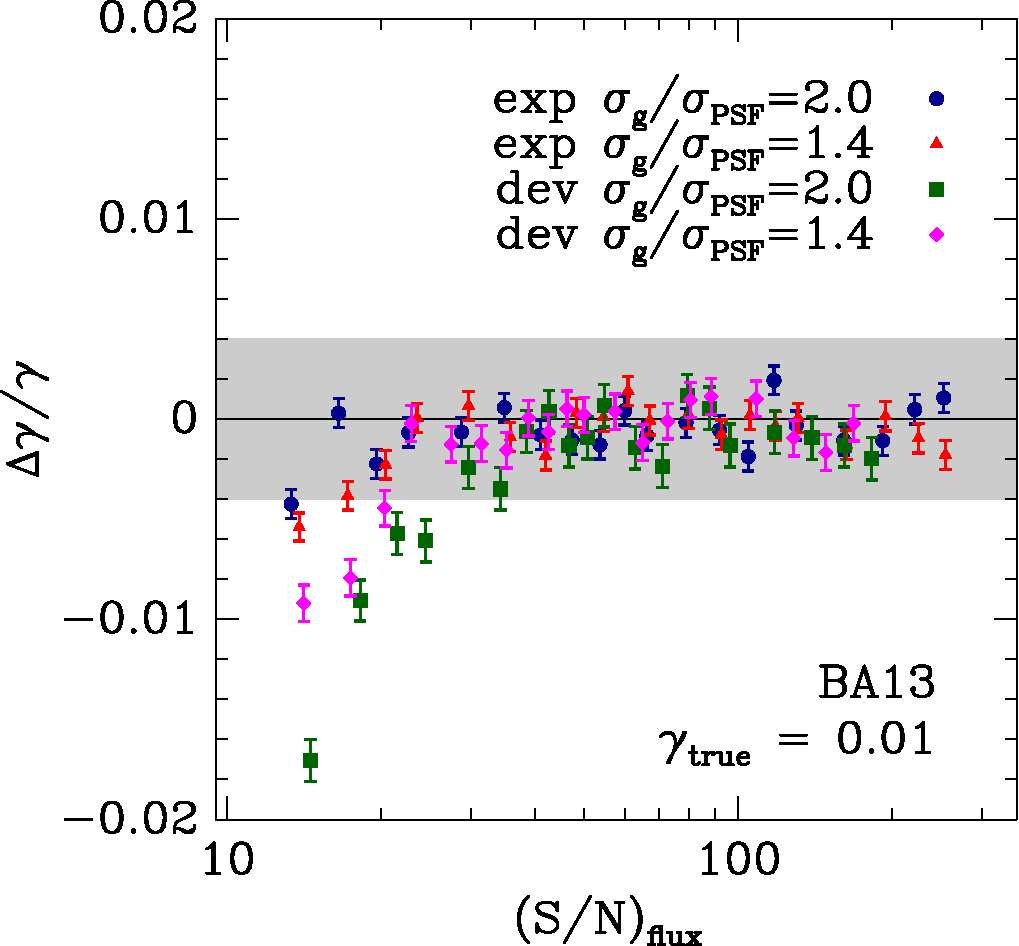
\includegraphics[width=\textwidth]{cbafit-geg07-geg08-deg03-deg05-ba13-flux-s2n.pdf}
        \end{column}

        \begin{column}{0.5\textwidth}
            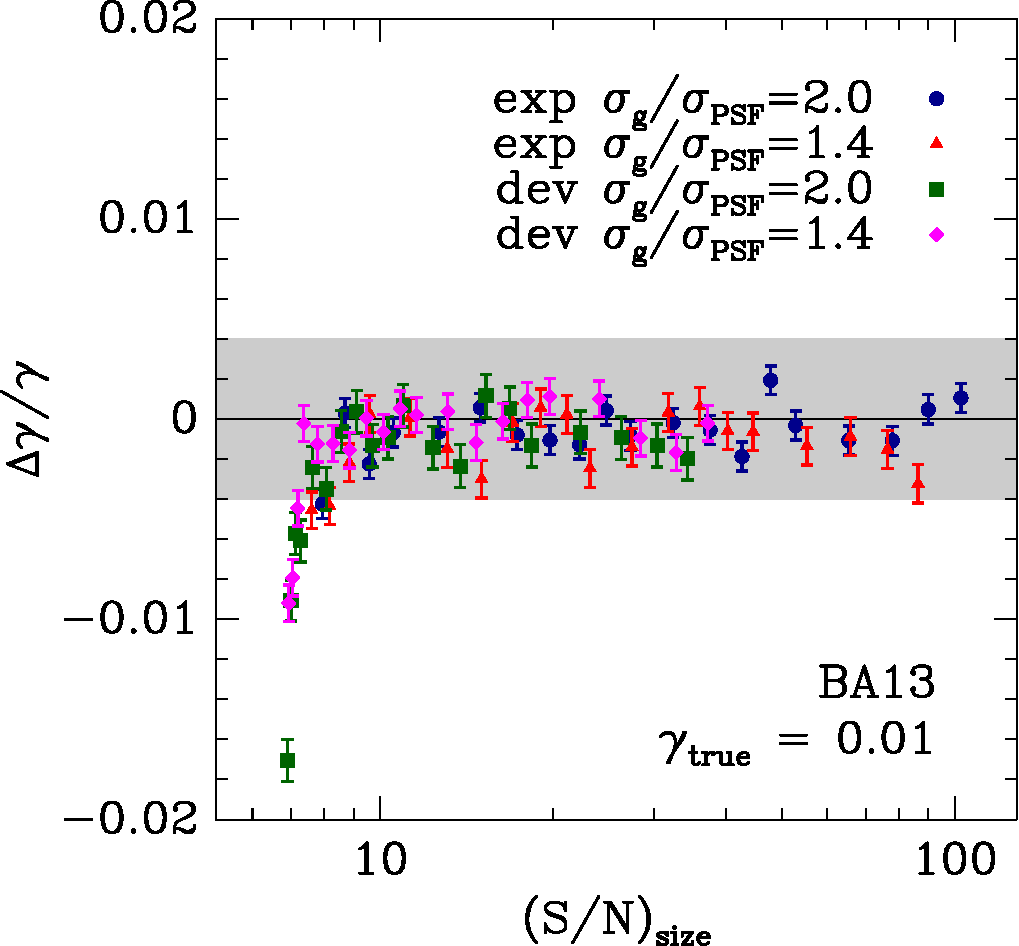
\includegraphics[width=\textwidth]{cbafit-geg07-geg08-deg03-deg05-ba13-T-s2n.pdf}
        \end{column}
    \end{columns}

    \begin{itemize}
        \item Assuming we can find the right model.
        \item Sufficient accuracy for DES at \snT$ > 10$.
    \end{itemize}
}


\frame{
    
    \frametitle{Bernstein \& Armstrong 2013 Tests}

    \begin{itemize}
        \item Can push to lower \snT\ than LENSFIT.

        \item Bias varies with \snT\ in a simpler way than LENSFIT.
        \item Bias vs \snT\ even more universal. Sufficient accuracy for DES at \snT$ > 10$.

       

    \end{itemize}
}

\frame{
    \frametitle{Limitations}
    \begin{itemize}

        \item I'm assuming I can find the right model.  Not true in real data.
            Should be OK for DES (Kacprzak et al. 2013) but not LSST.

        \item TODO: 
            
            \begin{itemize}

                \item Explore more realistic intrinsic distributions in
                    structural parameters (size, flux).  E.g. for a bin in {\it
                    measured} flux, what are the {\it true} distributions in
                    size and flux?  Use Cosmos.

                \item Why is there bias at all?  Is it the likelhood sampling method?

                \item Bernstein \& Armstrong propose a model-independent
                    technique using moments in Fourier space, but not yet
                    implemented.  Gary and Bob plan to do it.  Student at Stony
                    Brooke as well (Madhavacheril).

            \end{itemize}

    \end{itemize}
}

\frame{
    \frametitle{Summary}

    \begin{itemize}

        \item Shear estimation is difficult in the presence of noise.

        \item Modern techniques can work well enough for current surveys.

        \item For future experiments such as LSST we need a model-independent
            approach.

    \end{itemize}
}
\end{comment}

\end{document}
